
\newcommand{\insertFigCompToy}{
\begin{figure}
\centering
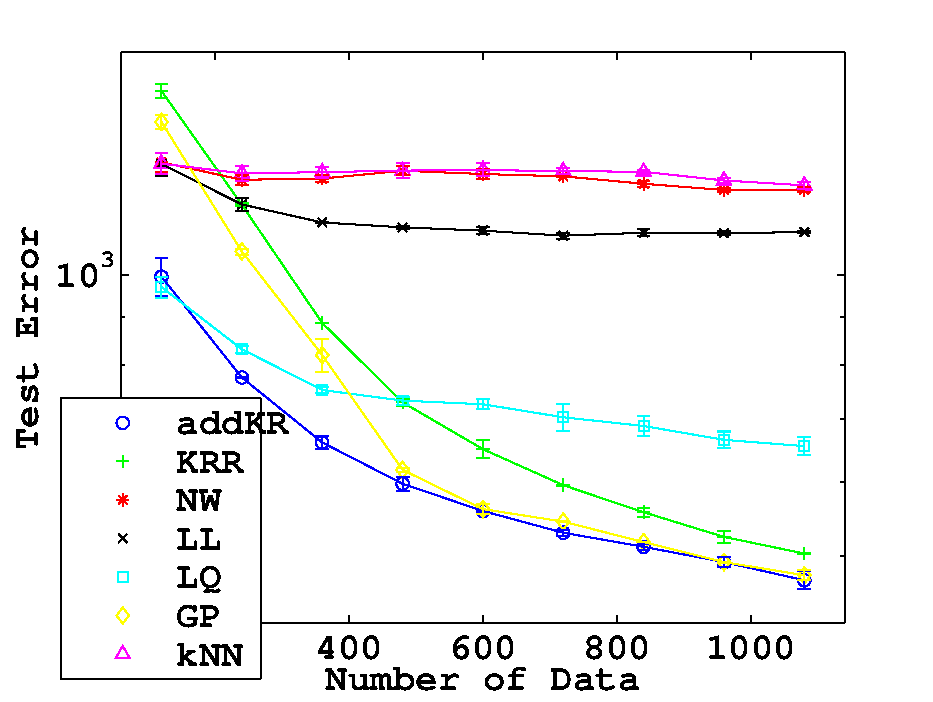
\includegraphics[width=3.2in]{figs/compToy}
\vspace{\imcaptionspace}
\caption[]{\small Comparison of various nonparametric regression methods on a
$20$-dimensional toy dataset. The $x$-axis denotes the number of training data
and the $y$-axis is the test error. }
\vspace{\imtextspace}
\label{fig:compToy}
\end{figure}
}


\newcommand{\insertFigSolnPath}{
\begin{figure}
\centering
% 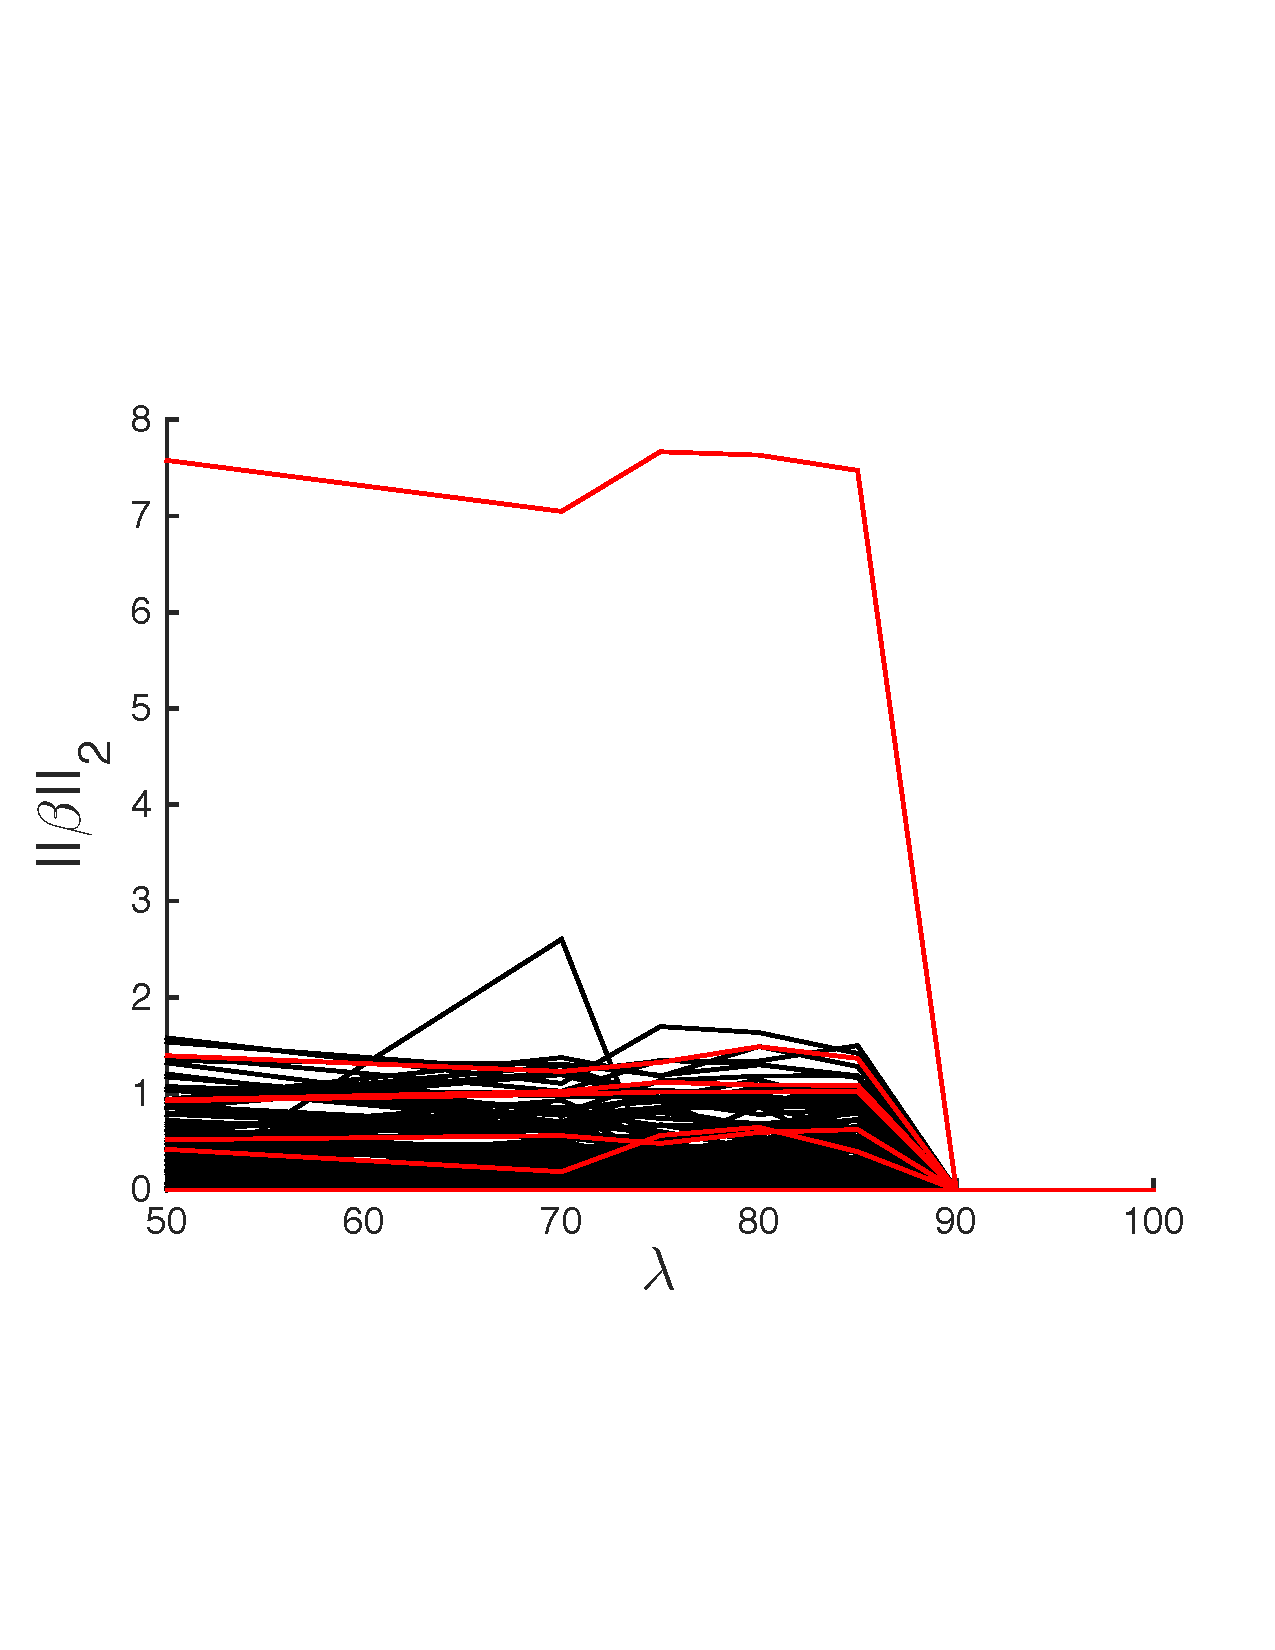
\includegraphics[width=3.4in]{figs/solnpath200.pdf}
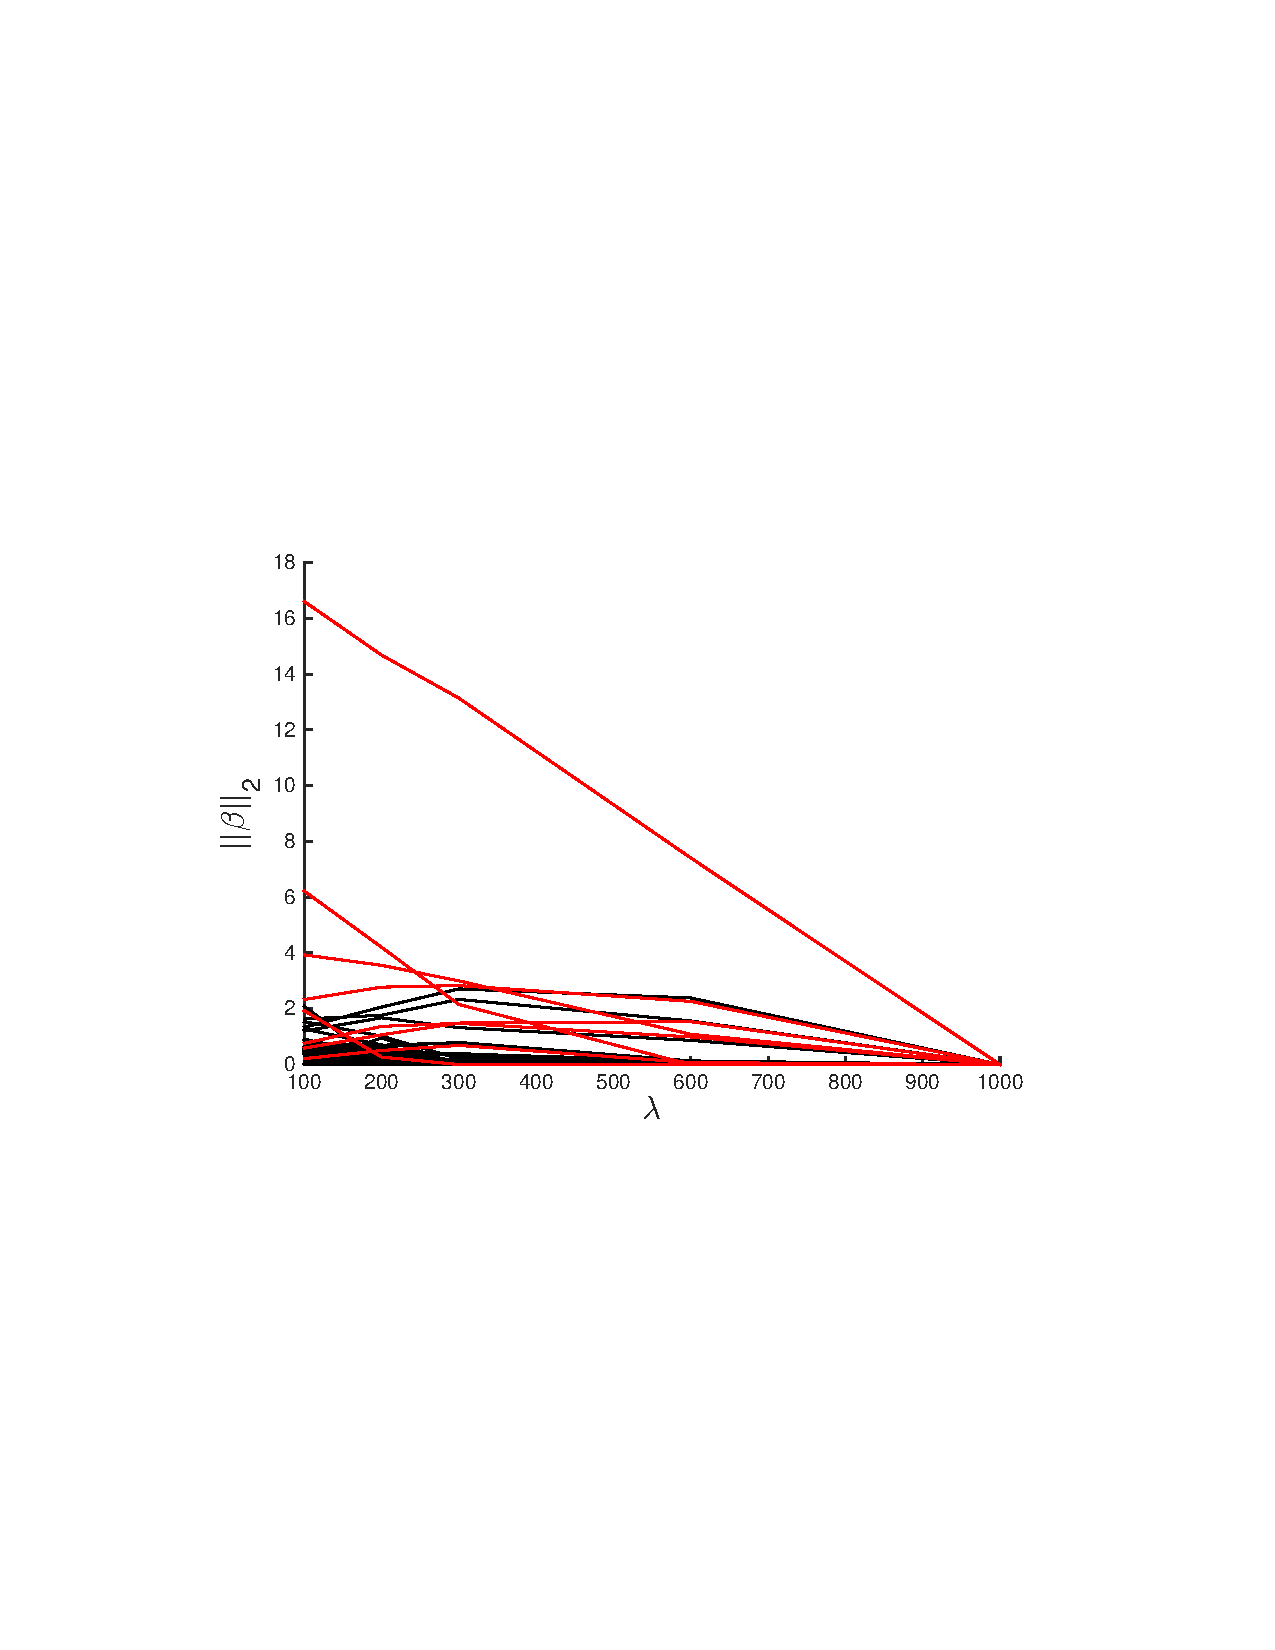
\includegraphics[width=3.2in]{figs/solnpath600.pdf}
\vspace{\imcaptionspace}
\caption[]{\small Solution path with $n=200$ samples (above) and
$n=600$ (below). The $x$-axis shows the regularization parameter,
while the $y$-axis plots $\|\funcj\|_{\Hcalkj} = \|\betaj\|$. 
The true nonzero functiosn are depicted in red. As the figure indicates, several
of the false functions are driven to $0$ fast whereas the true functions
persist for longer.
}
\vspace{\imtextspace}
\label{fig:n200}
\end{figure}
}
